\chapter{Usare Sphinx per creare la documentazione}

\textbf{Nota:} ho seguito fondamentalmente le istruzioni scritte nei tutorial ai seguenti link:\\
\url{https://shunsvineyard.info/2019/09/19/use-sphinx-for-python-documentation/}\\
\url{https://towardsdatascience.com/documenting-python-code-with-sphinx-554e1d6c4f6d}\\

Sphinx provides two command-line tools: sphinx-quickstart and sphinx-apidoc.
\begin{enumerate}
    \item \textbf{\texttt{sphinx-quickstart}} sets up a source directory and creates a default configuration, conf.py, and a master document, index.rst, which serves as a welcome page of a document.
    \item \textbf{\texttt{sphinx-apidoc}} generates reStructuredText files to document from all found modules.
\end{enumerate}
\noindent
Il workflow tipico può essere rapprensetato nel seguente diagramma:

\begin{figure}[ht]
    \centering
    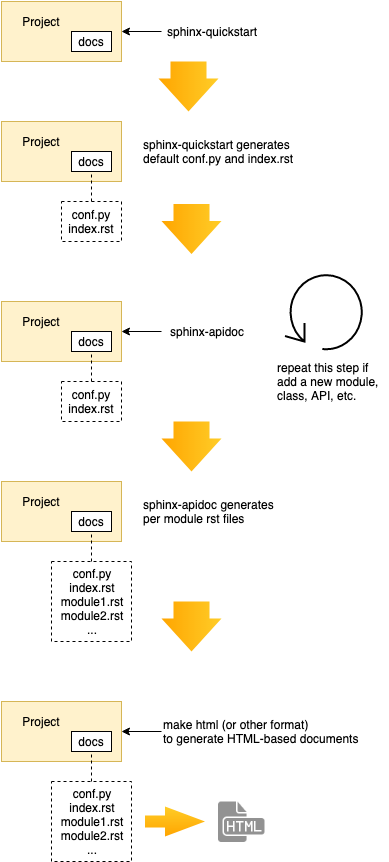
\includegraphics[width=0.53\textwidth]{images/sphinx_workflow.png}
\end{figure}
\FloatBarrier

\subsection{Step 1: Use sphinx-quickstart to generate Sphinx source directory with conf.py and index.rst}

Supponiamo che il nostro progetto abbia la seguente struttura:
\begin{minted}{bash}
sphinx_basics
 |- docs
 |- maths
    |- add.py
    |- divide.py
    |- multiply.py
    |- subtract.py
    |- __init__.py
\end{minted}
Vogliamo mettere tutta la documentazione nella cartella \texttt{docs}.\\
Per farlo ci mettiamo nella cartella \texttt{docs} e scriviamo:

\begin{minted}{bash}
 sphinx-quickstart
\end{minted}

Ci varranno chieste alcune domande riguardo al nostro progetto. In particolare, rispondere \texttt{(y)} alla domanda:

\begin{minted}{bash}
 > Separate source and build directories (y/n) [n]: y
\end{minted}

A questo punto la cartella \texttt{docs} avrà una struttura del genere:

\begin{minted}{bash}
docs
-- Makefile
-- build
-- make.bat
-- source
    |- _static
    |- _templates
    |- conf.py
    |- index.rst
\end{minted}

\subsection{Step 2: Configure the conf.py}

sphinx-quickstart generates a few files, and the most important one is conf.py, which is the configuration of the documents. Although conf.py serves as a configuration file, it is a real Python file. The content of conf.py is Python syntax.\\

Go to your conf.py file and uncomment line numbers 13,14 and 15. Change the \texttt{os.path.abspath('.')} to \texttt{os.path.abspath('..')}. Here, we tell sphinx that the code is residing outside of the current docs folder.\\

Per far funzionare le cose, puoi direttamente copiare e incollare il seguente script:

\inputminted{python}{conf.py}


\subsection{Step 3: Use sphinx-apidoc to generate reStructuredText files from source code}

A questo punto, andiamo nella cartella madre del nostro progetto (\texttt{sphinx\_basics}) e scriviamo (con le sostituzioni opportune):

\begin{minted}{bash}
sphinx-apidoc -f -o <path-to-output> <path-to-module>
\end{minted}

-f means force overwriting of any existing generated files.\\
-o means the path to place the output files.

Nel caso preso in esempio, scriviamo:

\begin{minted}{bash}
sphinx-apidoc -f -o docs maths/
\end{minted}


\subsection{Step 4: Including module.rst and generating html}

The generated \texttt{modules.rst} contains all the modules. So we need to add the \texttt{modules.rst} to \texttt{index.rst}.

Apriamo il file (\texttt{index.rst}) e scriviamo \texttt{modules} come nel seguente esempio:

\begin{minted}{bash}
.. toctree::
   :maxdepth: 2
   :caption: Contents:

   modules
\end{minted}

%per aggiungere anche il file readme guarda https://towardsdatascience.com/documenting-python-code-with-sphinx-554e1d6c4f6d

A questo punto tutto è pronto per generare la nostra documentazione. Andiamo nella cartella \texttt{docs} e scriviamo:

\begin{minted}{bash}
make html
\end{minted}

Ecco fatto! Abbiamo generato la nostra documentazione nella cartella \texttt{\_build}